%%%%%%%%%%%%%%%%%%%%%%%%%%%%%%%%%%%%%%%%%%%%%%%%%%%%%%%%%%%%%%%%%%%%%
% LaTeX Template: Project Titlepage Modified (v 0.1) by rcx
%
% Original Source: http://www.howtotex.com
% Date: February 2014
% 
% This is a title page template which be used for articles & reports.
% 
% This is the modified version of the original Latex template from
% aforementioned website.
% 
%%%%%%%%%%%%%%%%%%%%%%%%%%%%%%%%%%%%%%%%%%%%%%%%%%%%%%%%%%%%%%%%%%%%%%

\documentclass[12pt]{report}
\usepackage[a4paper]{geometry}
\usepackage[myheadings]{fullpage}
\usepackage{fancyhdr}
\usepackage{lastpage}
\usepackage{graphicx, wrapfig, subcaption, setspace, booktabs}
\usepackage[T1]{fontenc}
\usepackage[font=small, labelfont=bf]{caption}
\usepackage{fourier}
\usepackage[protrusion=true, expansion=true]{microtype}
\usepackage[english]{babel}
\usepackage{sectsty}
\usepackage{url, lipsum}
\usepackage{hyperref}
\usepackage{listings}
\usepackage{scrextend}
\usepackage{tikz}
\usepackage[]{algorithm2e}
\usepackage{float}
\usepackage{mathtools}
\usepackage{tabularx}
\usepackage{csquotes}
\usepackage{amssymb}
\usetikzlibrary{arrows}
\usetikzlibrary{arrows.meta}
\addtokomafont{labelinglabel}{\sffamily}


\newcommand{\HRule}[1]{\rule{\linewidth}{#1}}
\onehalfspacing
\setcounter{tocdepth}{5}
\setcounter{secnumdepth}{5}

%-------------------------------------------------------------------------------
% HEADER & FOOTER
%-------------------------------------------------------------------------------
\pagestyle{fancy}
\fancyhf{}
\setlength\headheight{15pt}
\fancyhead[L]{G52ACE}
\fancyhead[R]{University of Nottingham}
\fancyfoot[R]{Page \thepage\ of \pageref{LastPage}}
%-------------------------------------------------------------------------------
% TITLE PAGE
%-------------------------------------------------------------------------------

\begin{document}

\title{ \normalsize \textsc{}
		\\ [2.0cm]
		\HRule{0.5pt} \\
                \LARGE \textbf{\uppercase{Algorithms, Correctness \\and Efficiency\\G52ACE}}
		\HRule{2pt} \\ [0.5cm]
		\normalsize \today \vspace*{5\baselineskip}}

\date{}

\author{
		University of Nottingham\\
		Department of Computer Science }

\maketitle
\tableofcontents
\newpage

%-------------------------------------------------------------------------------
% Section title formatting
\sectionfont{\scshape}
%-------------------------------------------------------------------------------

%-------------------------------------------------------------------------------
% BODY
%-------------------------------------------------------------------------------

\section*{Introduction}
\addcontentsline{toc}{section}{Introduction}
Algorithms, Correctness and Efficiency is a 20 credit module. There are two exams. The first is on the 23\textsuperscript{rd} January 2017 and is worth 25\%. The second is in the summer and is worth 50\%.

\section*{Lecture 1: Analysing Algorithms}
\addcontentsline{toc}{section}{Analysing Algorithms}

\subsection*{What is an algorithm}
An algorithm is a step-by-step solution for solving a problem in a \textbf{finite} amount of time. Most algorithms convert input data to ouput data. The running time typically grows with the input size. The average running time of an algorithm is often very hard to calculate so we focus on the worst case. We often refer to the worst case as $T(n)$.

We can guess the running time through experimentation however this may not be accurate. It may also be time consuming. It is not possible if you want to know the running time ahead of computation. You will also have to implement the algorithm which won't be ideal if you want to evaluate algorithms before programming them in code.

Theoretical analysis of algorithms characterizes running time as a function of the runnign time \textbf{n}.

It is important to write the algorithm in pseudo code in order to analyse it. We assume that the algorithm runs on a RAM (Random Access Machine different to the memory in your computer) which is a theoretical computer with a CPU and an unlimited supply of memory. The RAM model is not representative of a real computer and has certain differences i.e. unlimited memory, each memory cell can hold an arbitrary number etc.

\begin{figure}[H]
    \centering
    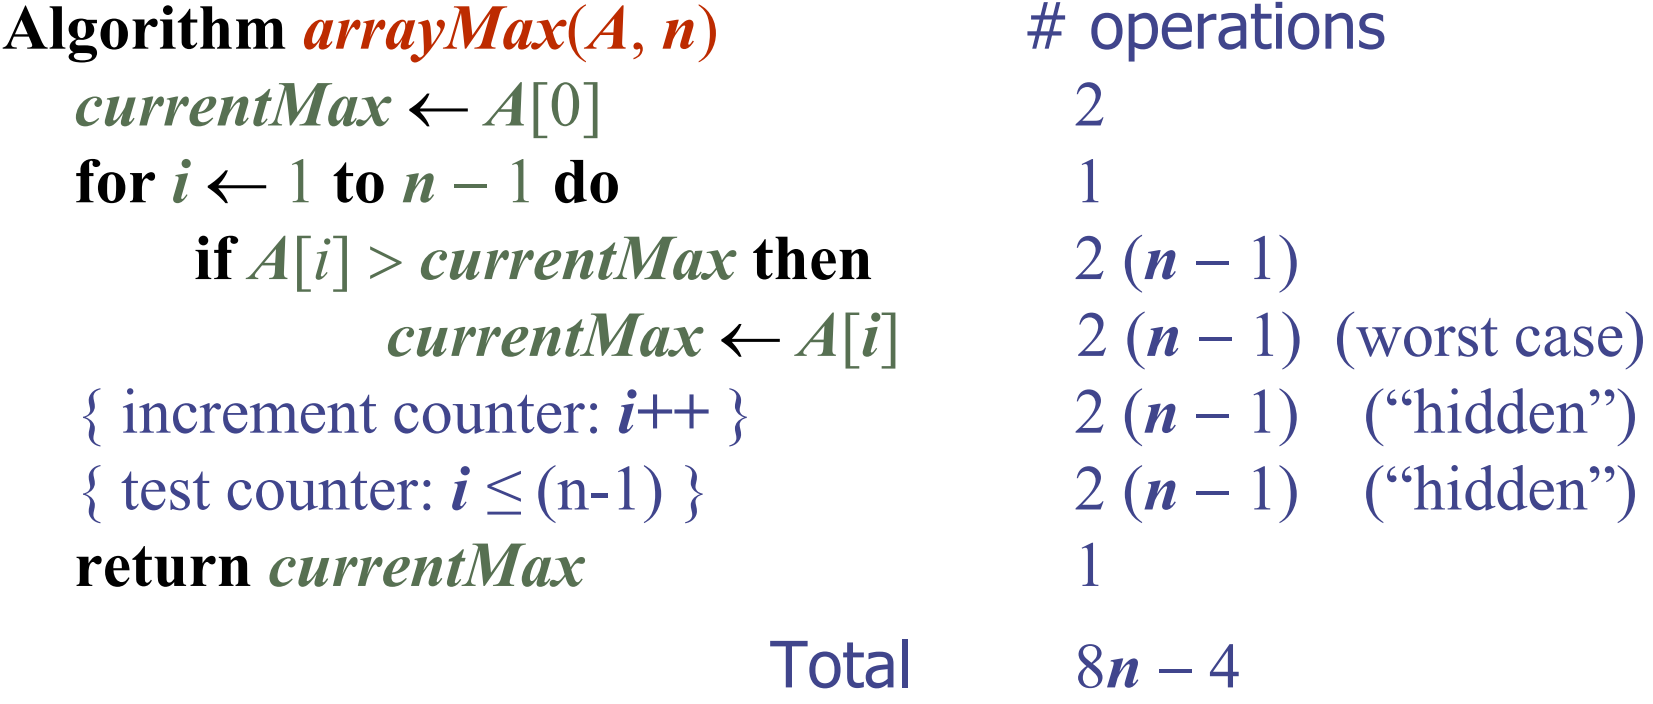
\includegraphics[width=0.75\textwidth]{images/arraymaxalgo.png}
    \caption{Counting primitive operations of an\\ algorithm calculating the largest number in an array}
\end{figure}

Unfortunately counting is quite vague. For example, one person might come up with 2 and another 4. Either could be correct but 2n will not be correct. Actual running time depends on many things including CPU architecture, RAM speed, compiler speed etc. It is impossible to take all these things into account so don't worry about finer details.

\end{document}

